\FloatBarrier
\subsection{Event selection}

\begin{figure}[ht]
    \begin{multicols}{2}
        \hfill
        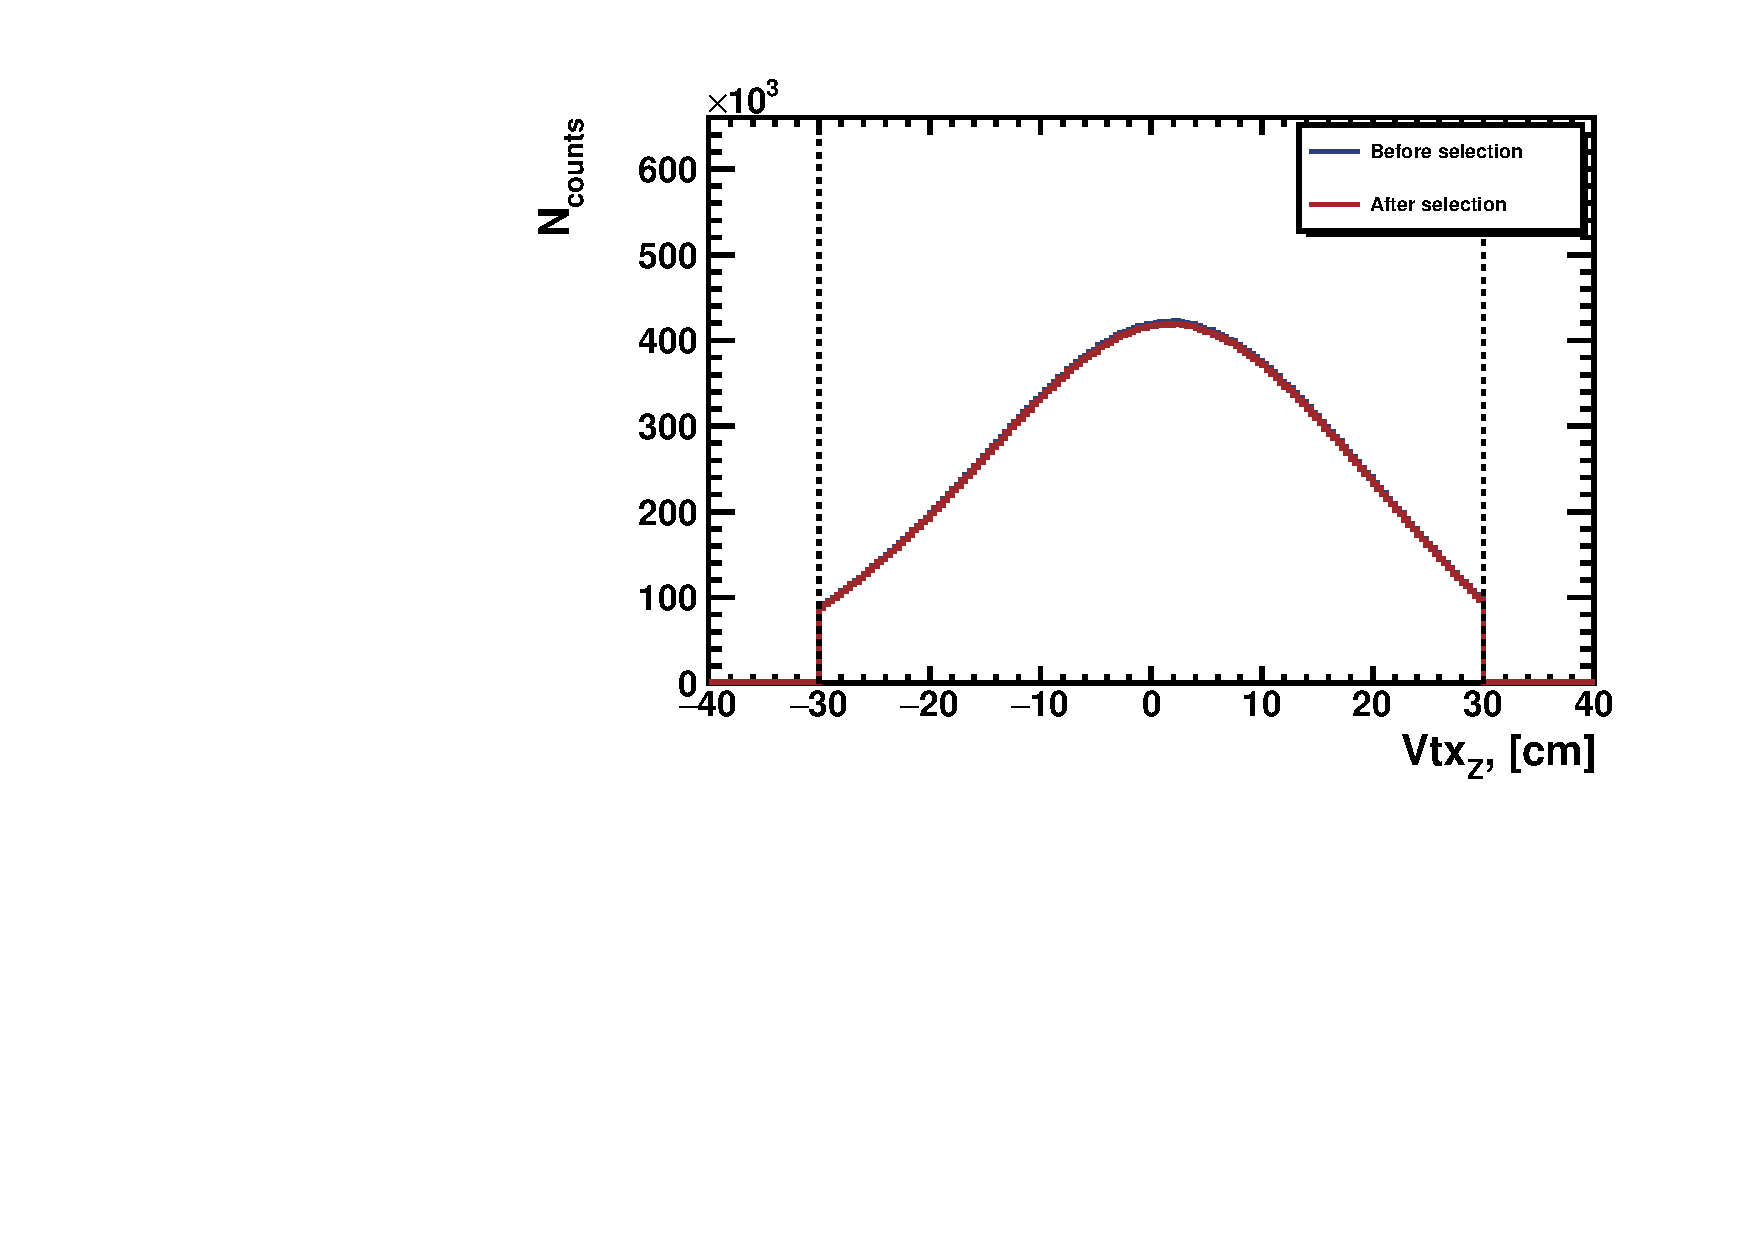
\includegraphics[width=0.49\textwidth]{Figures/VtxZ.pdf}
        \hfill
        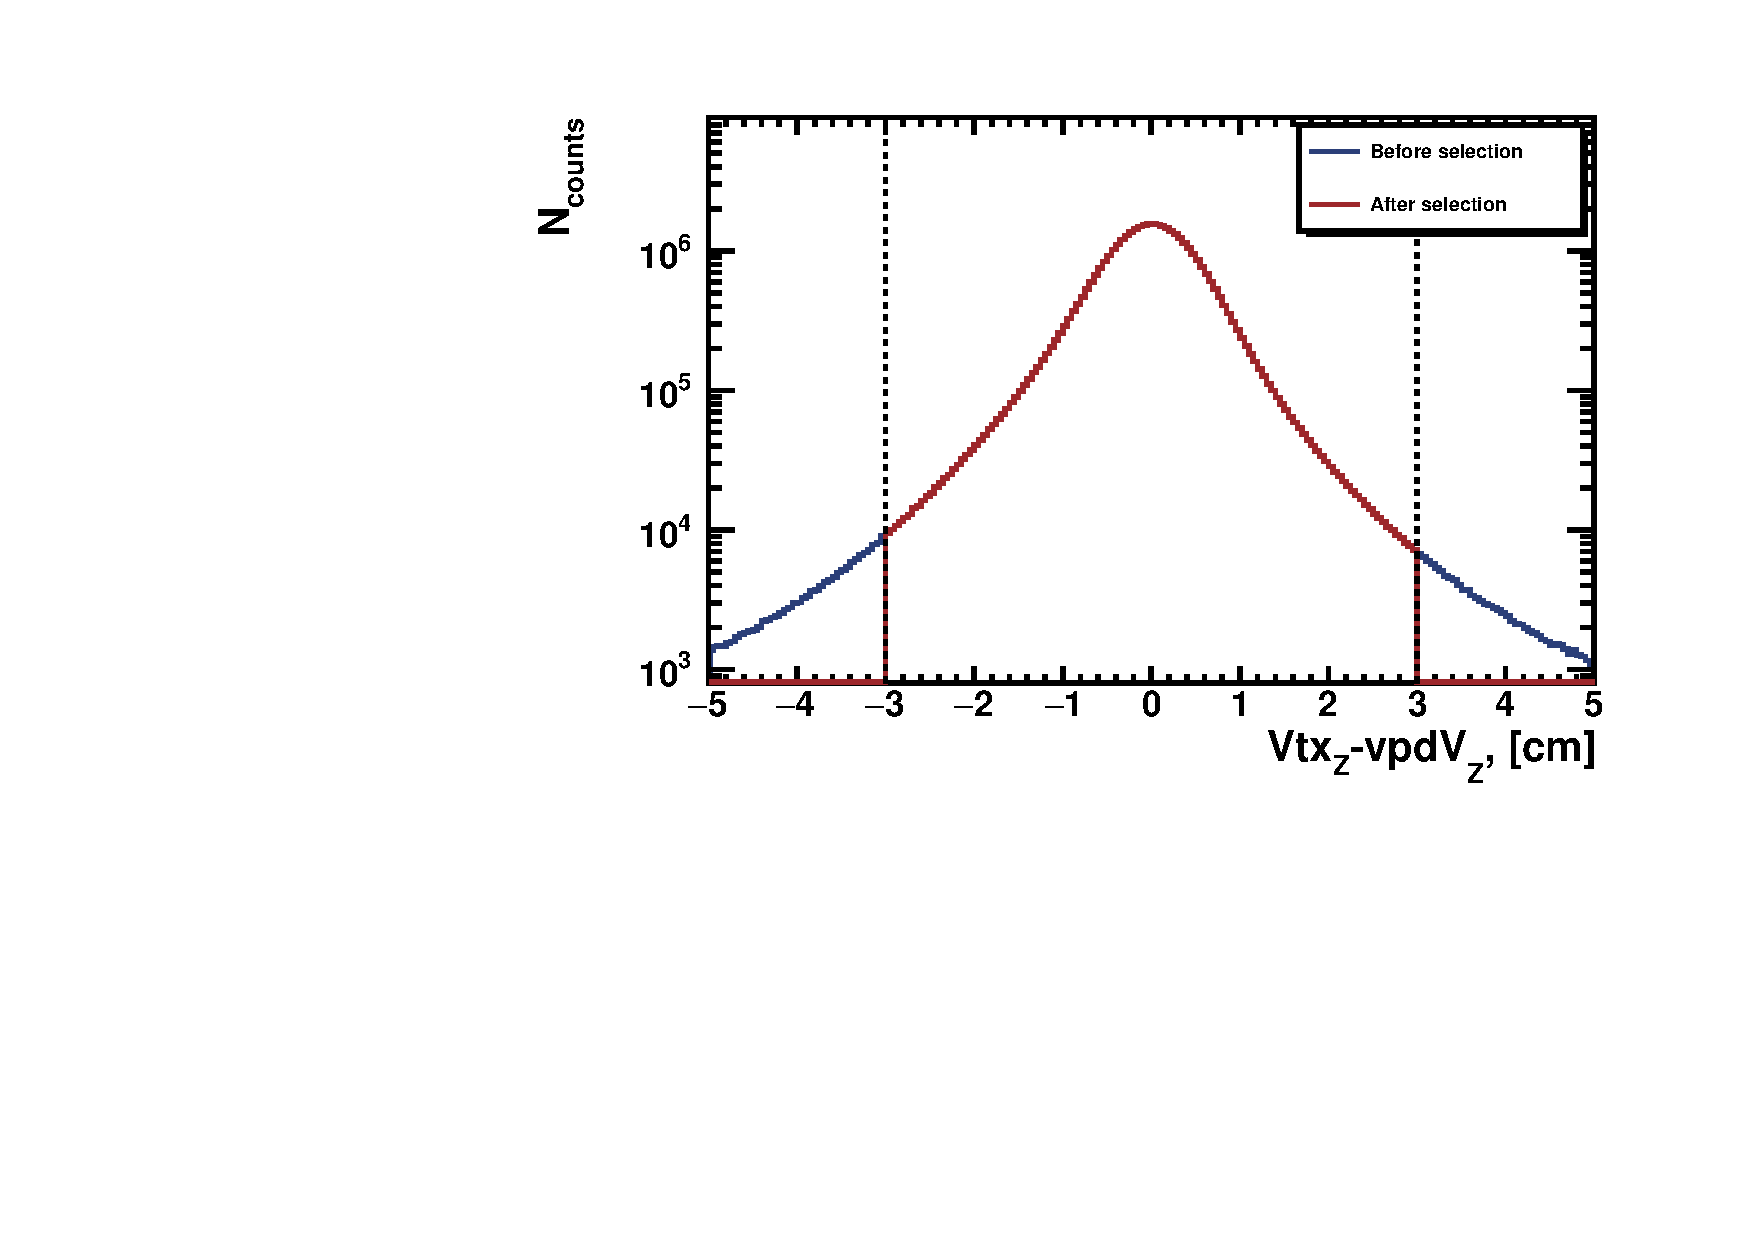
\includegraphics[width=0.49\textwidth]{Figures/VtxVpdZ.pdf}
    \end{multicols}
    \label{fig:VtxZCuts}
    \caption{Distribution of the $Vtx_Z$ (left) and $Vtx_Z - Vpd_Z$ (right).}
\end{figure}

\begin{figure}[ht]
    \begin{multicols}{2}
        \hfill
        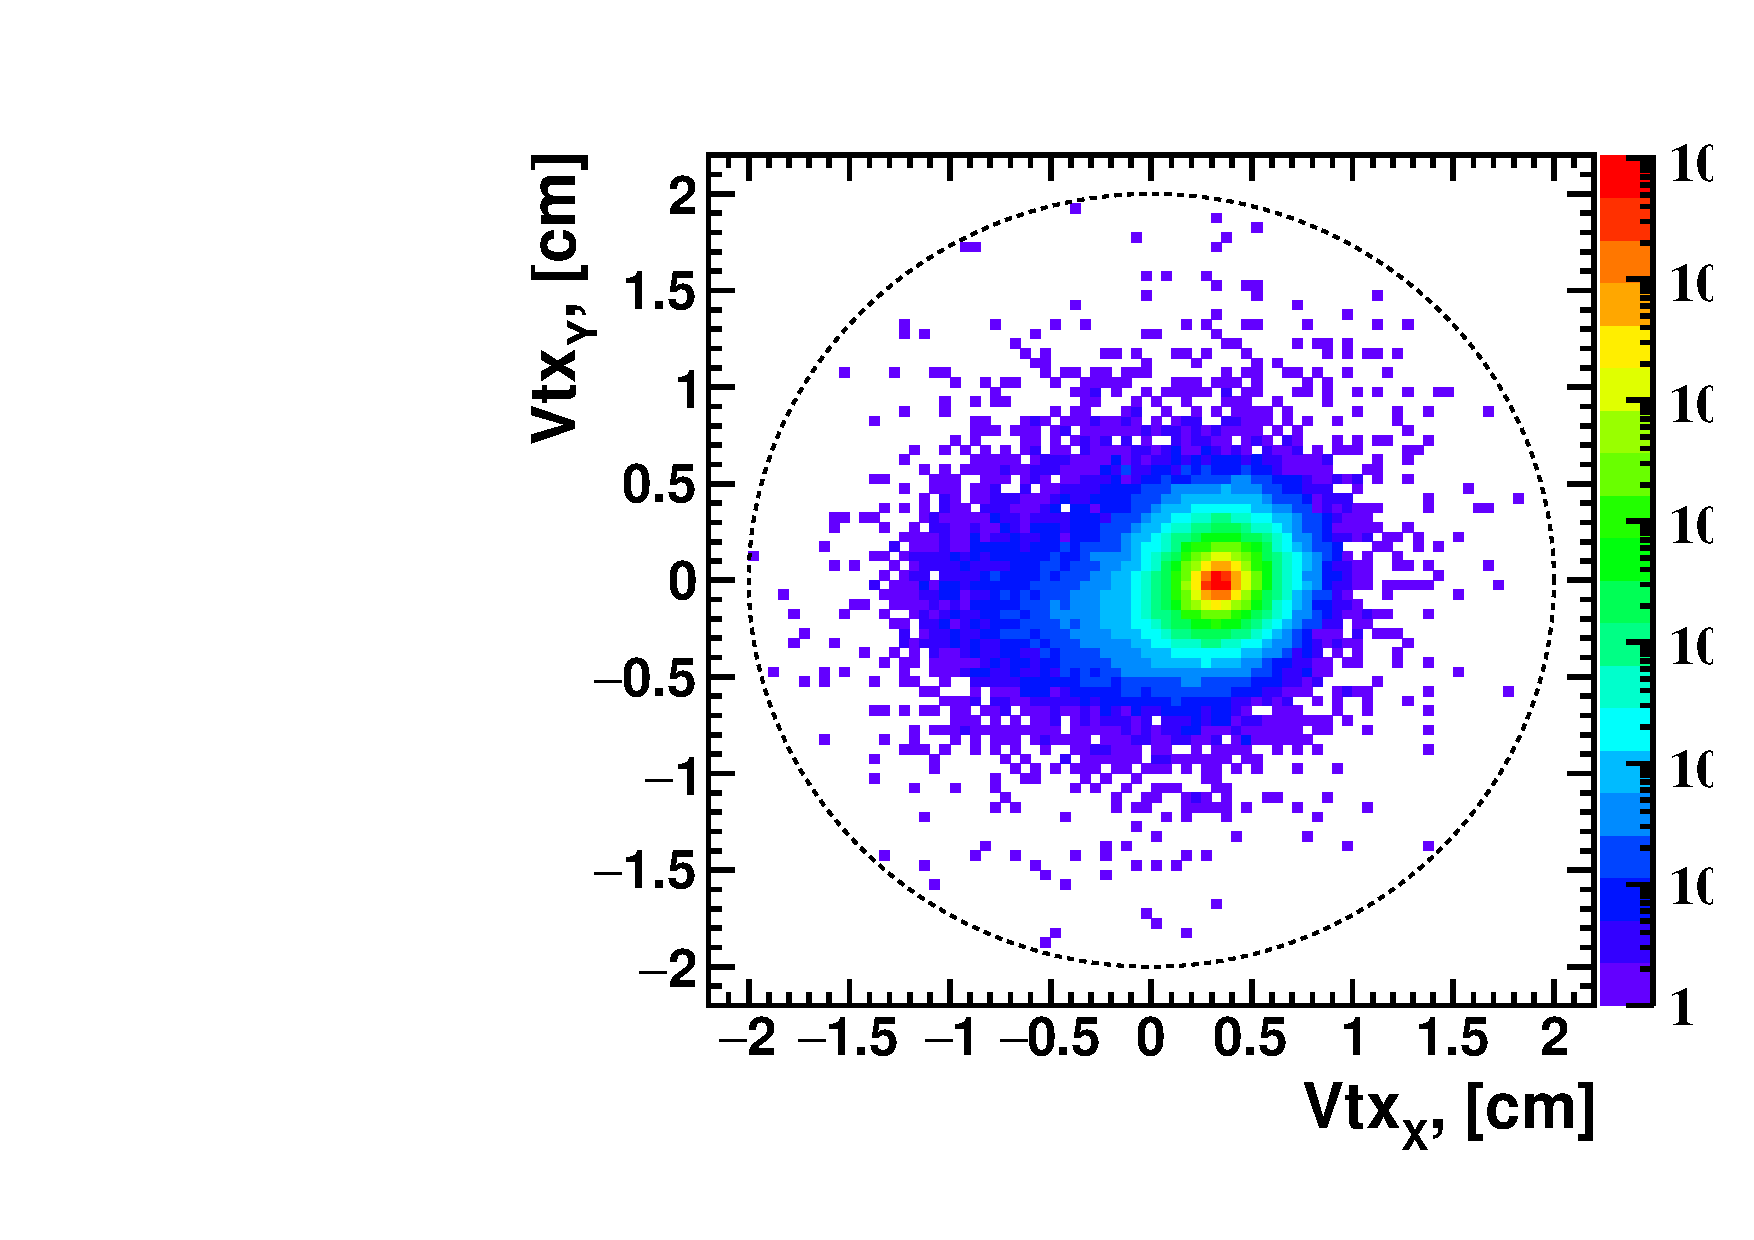
\includegraphics[width=0.49\textwidth]{Figures/VtxXY0.pdf}
        \hfill
        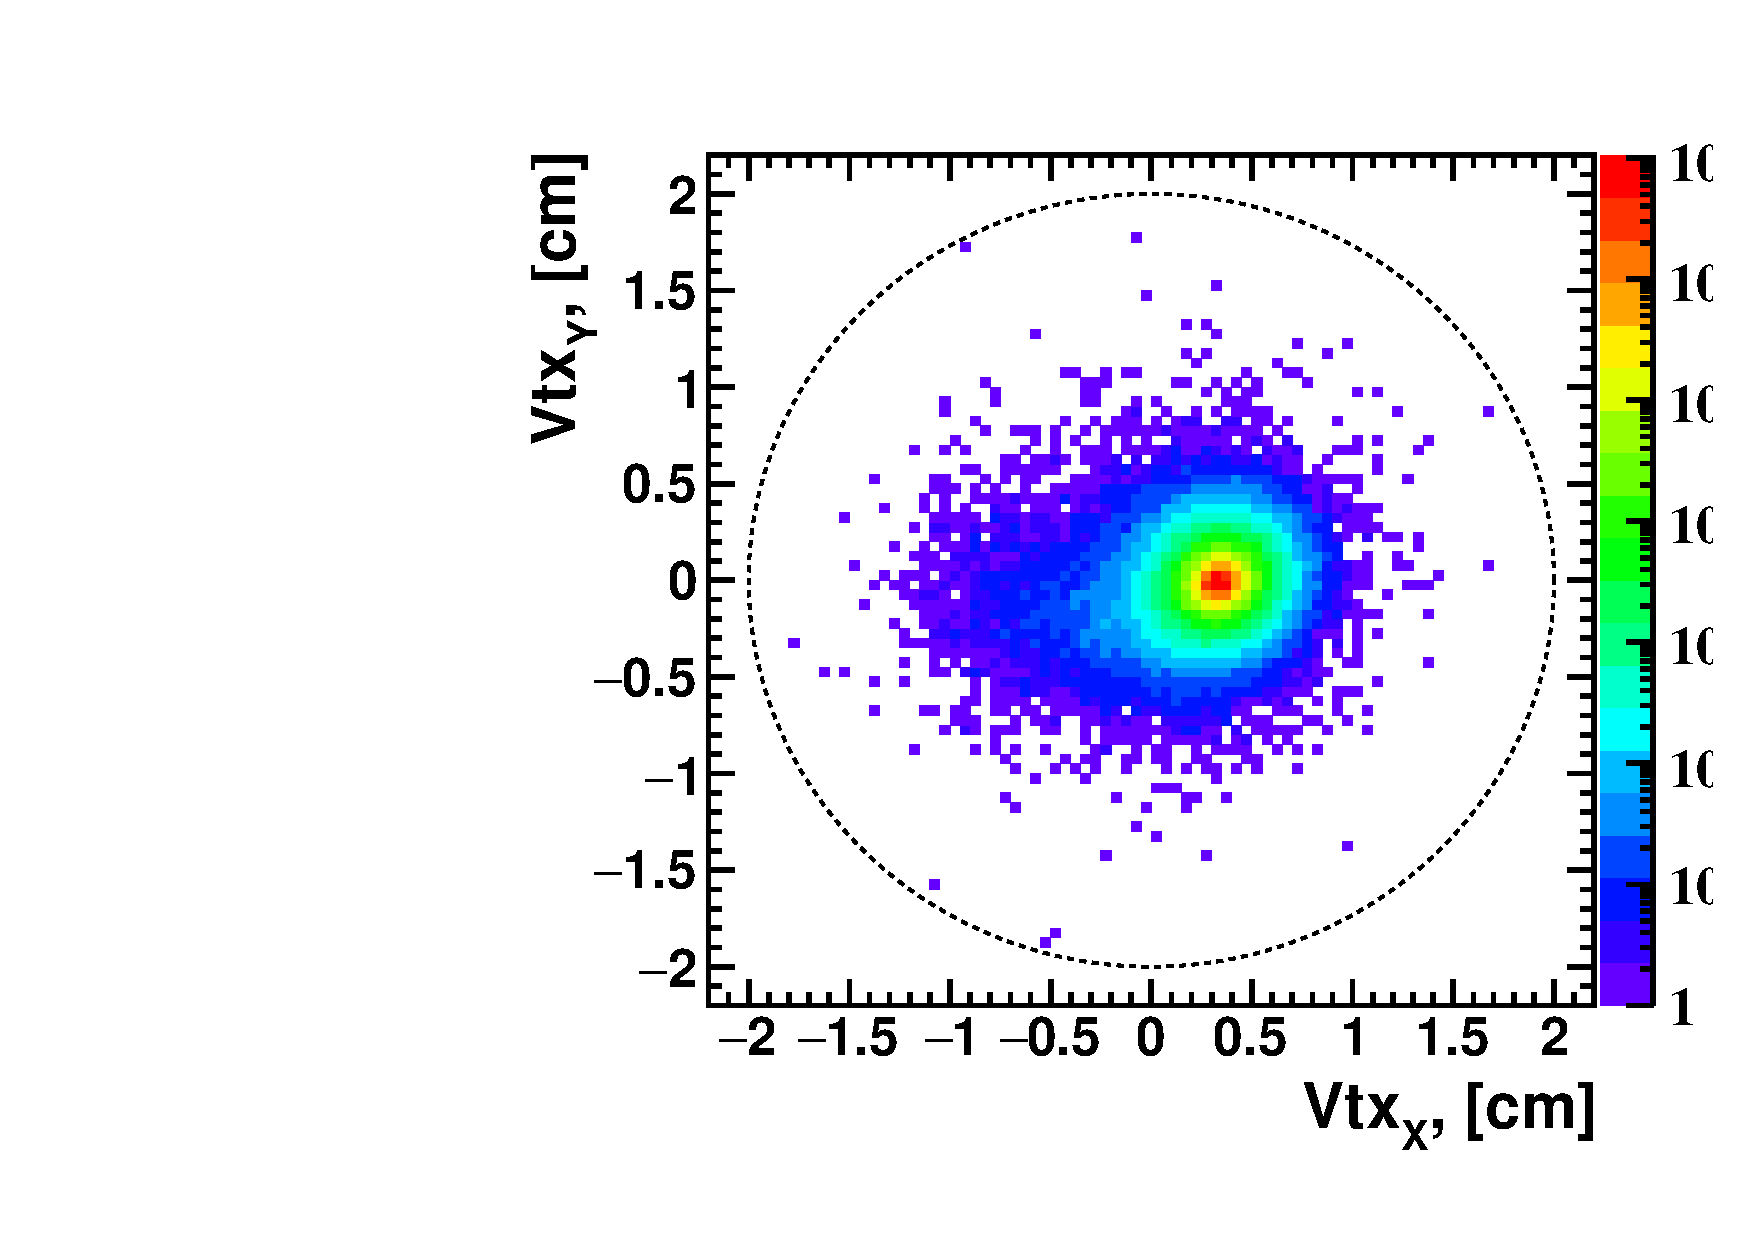
\includegraphics[width=0.49\textwidth]{Figures/VtxXY1.pdf}
    \end{multicols}
    \label{fig:VtxXYCuts}
    \caption{Distribution of the X-~and Y-components of the vertex before (left) and after (right) event selection.}
\end{figure}

\FloatBarrier
\subsection {Track selection}

\begin{figure}[ht]
    \begin{multicols}{2}
        \hfill
        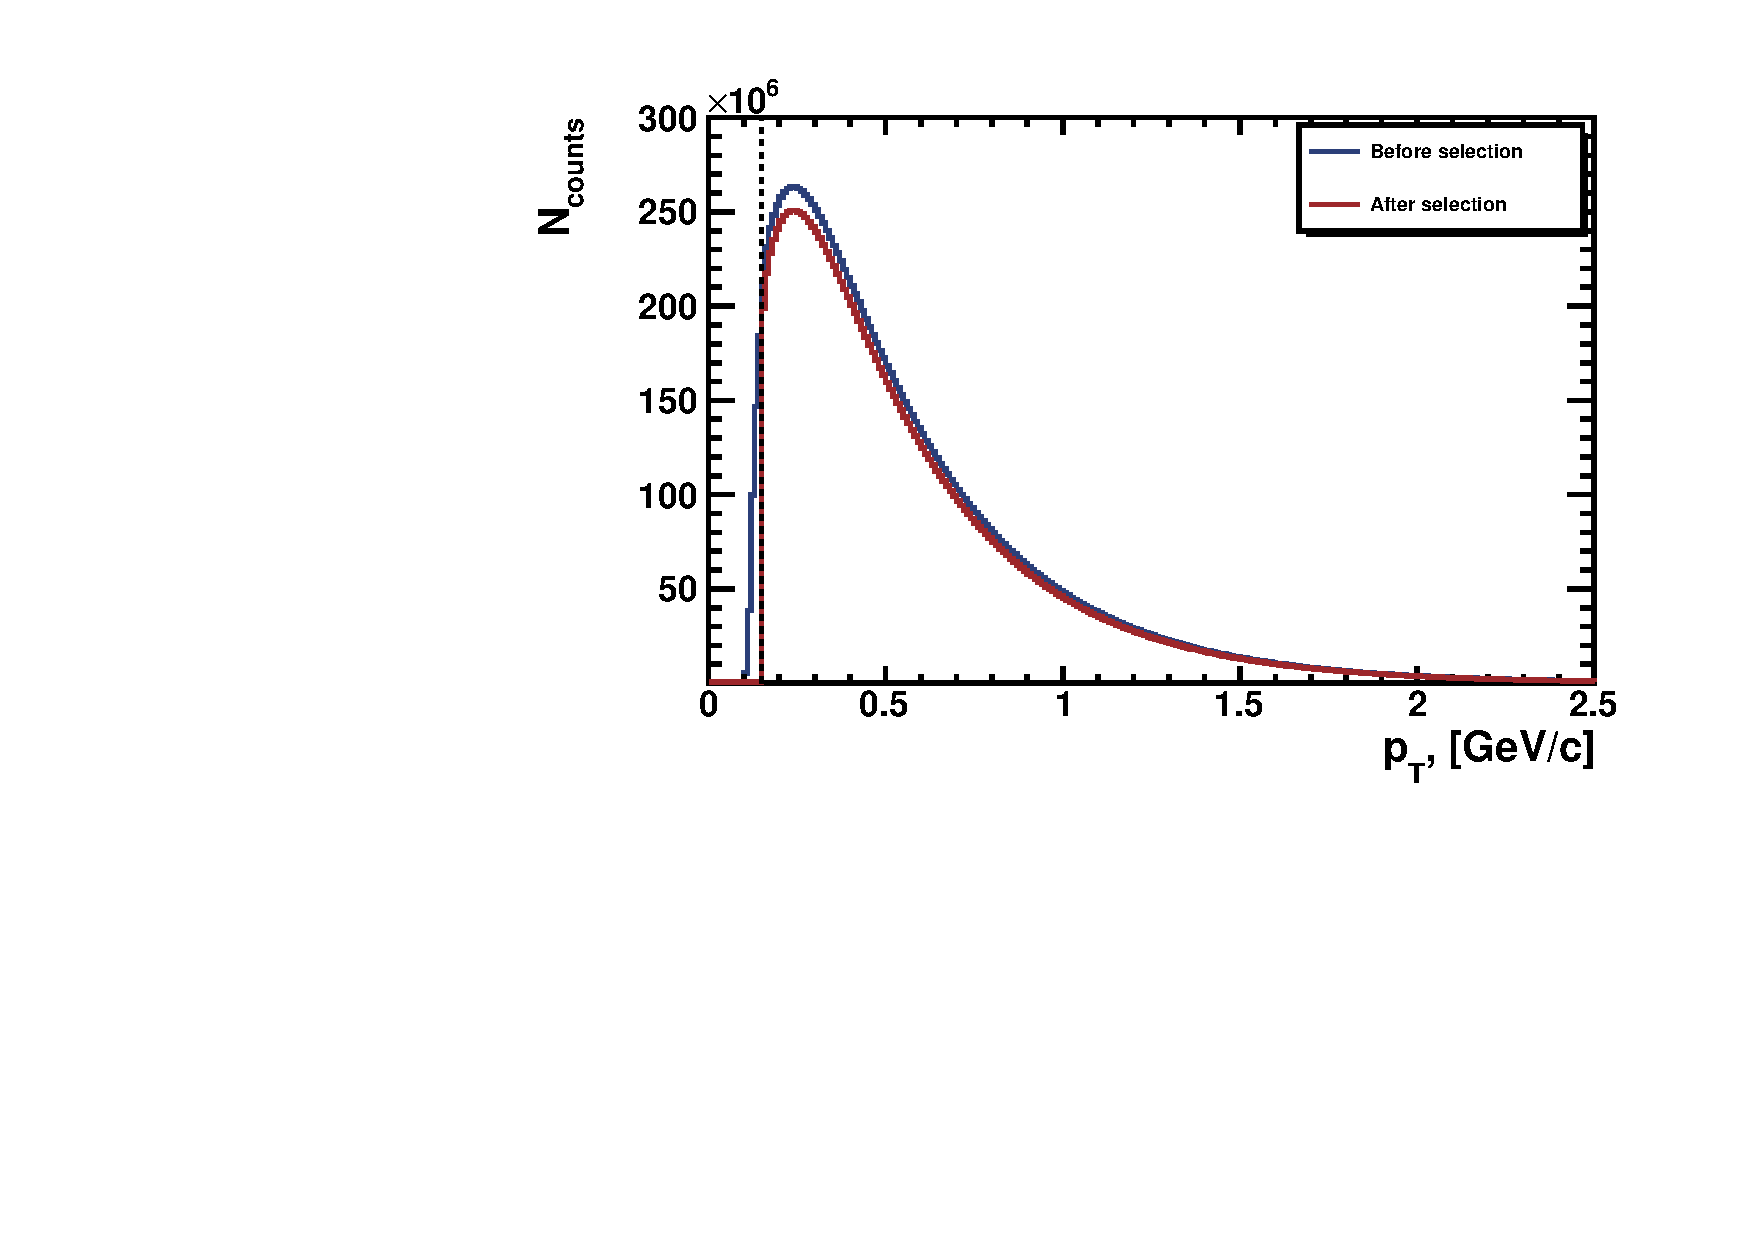
\includegraphics[width=0.49\textwidth]{Figures/Pt.pdf}
        \hfill
        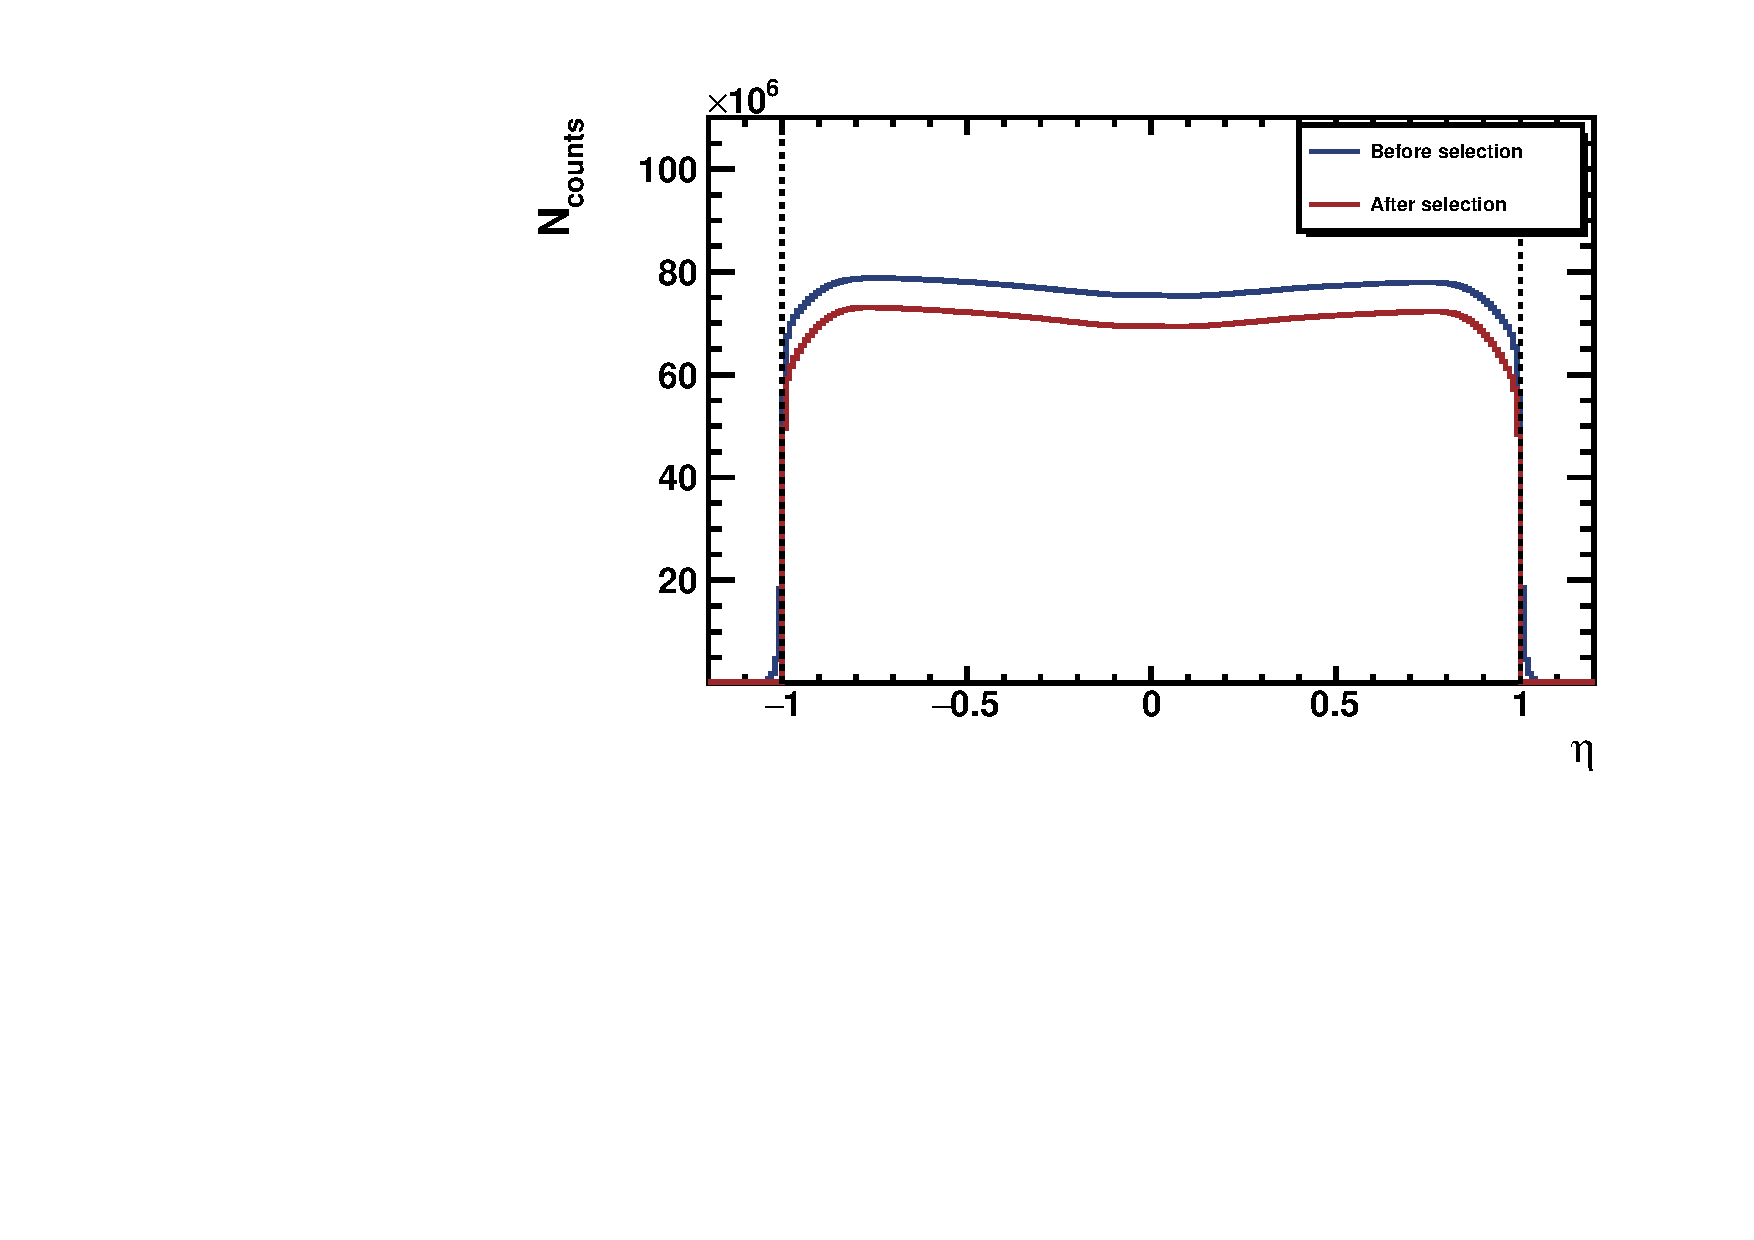
\includegraphics[width=0.49\textwidth]{Figures/Eta.pdf}
        \hfill
        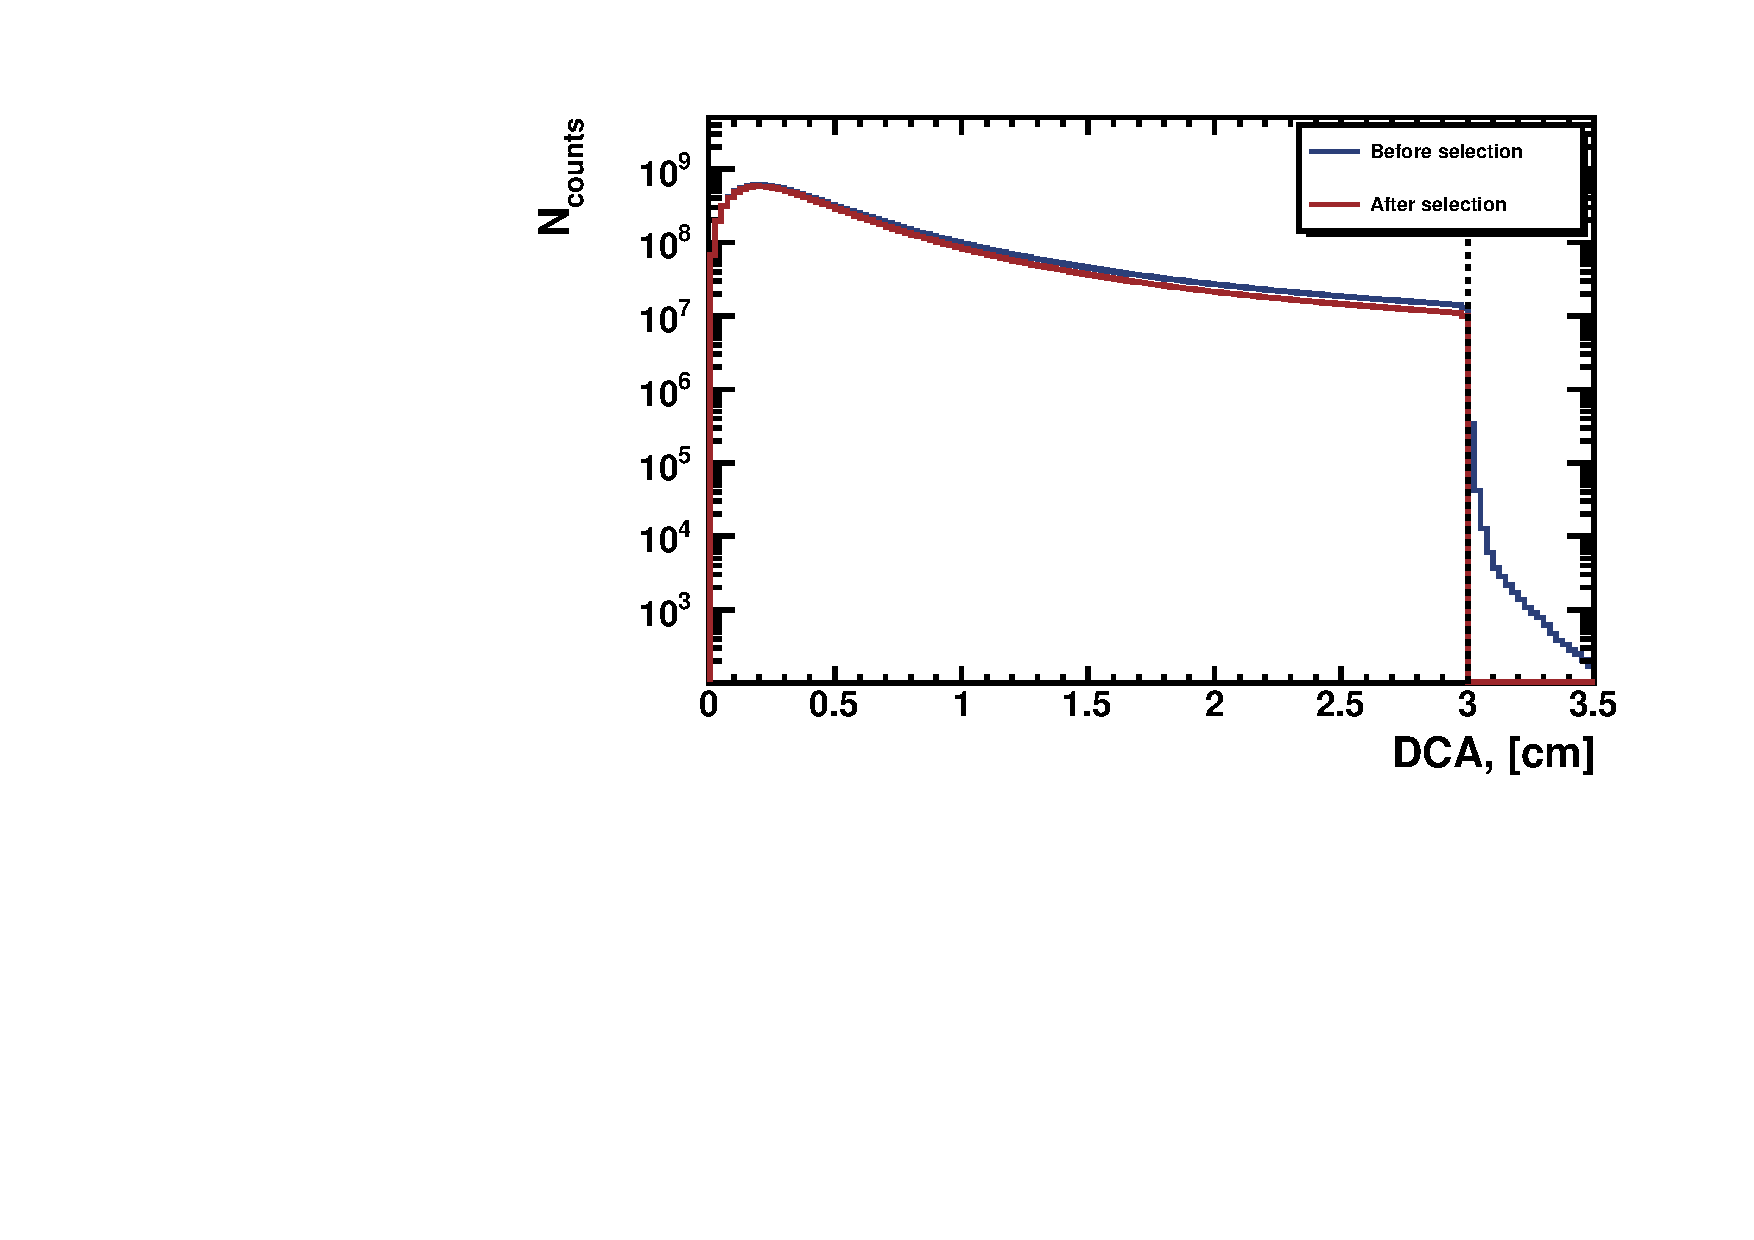
\includegraphics[width=0.49\textwidth]{Figures/DCA.pdf}
        \hfill
        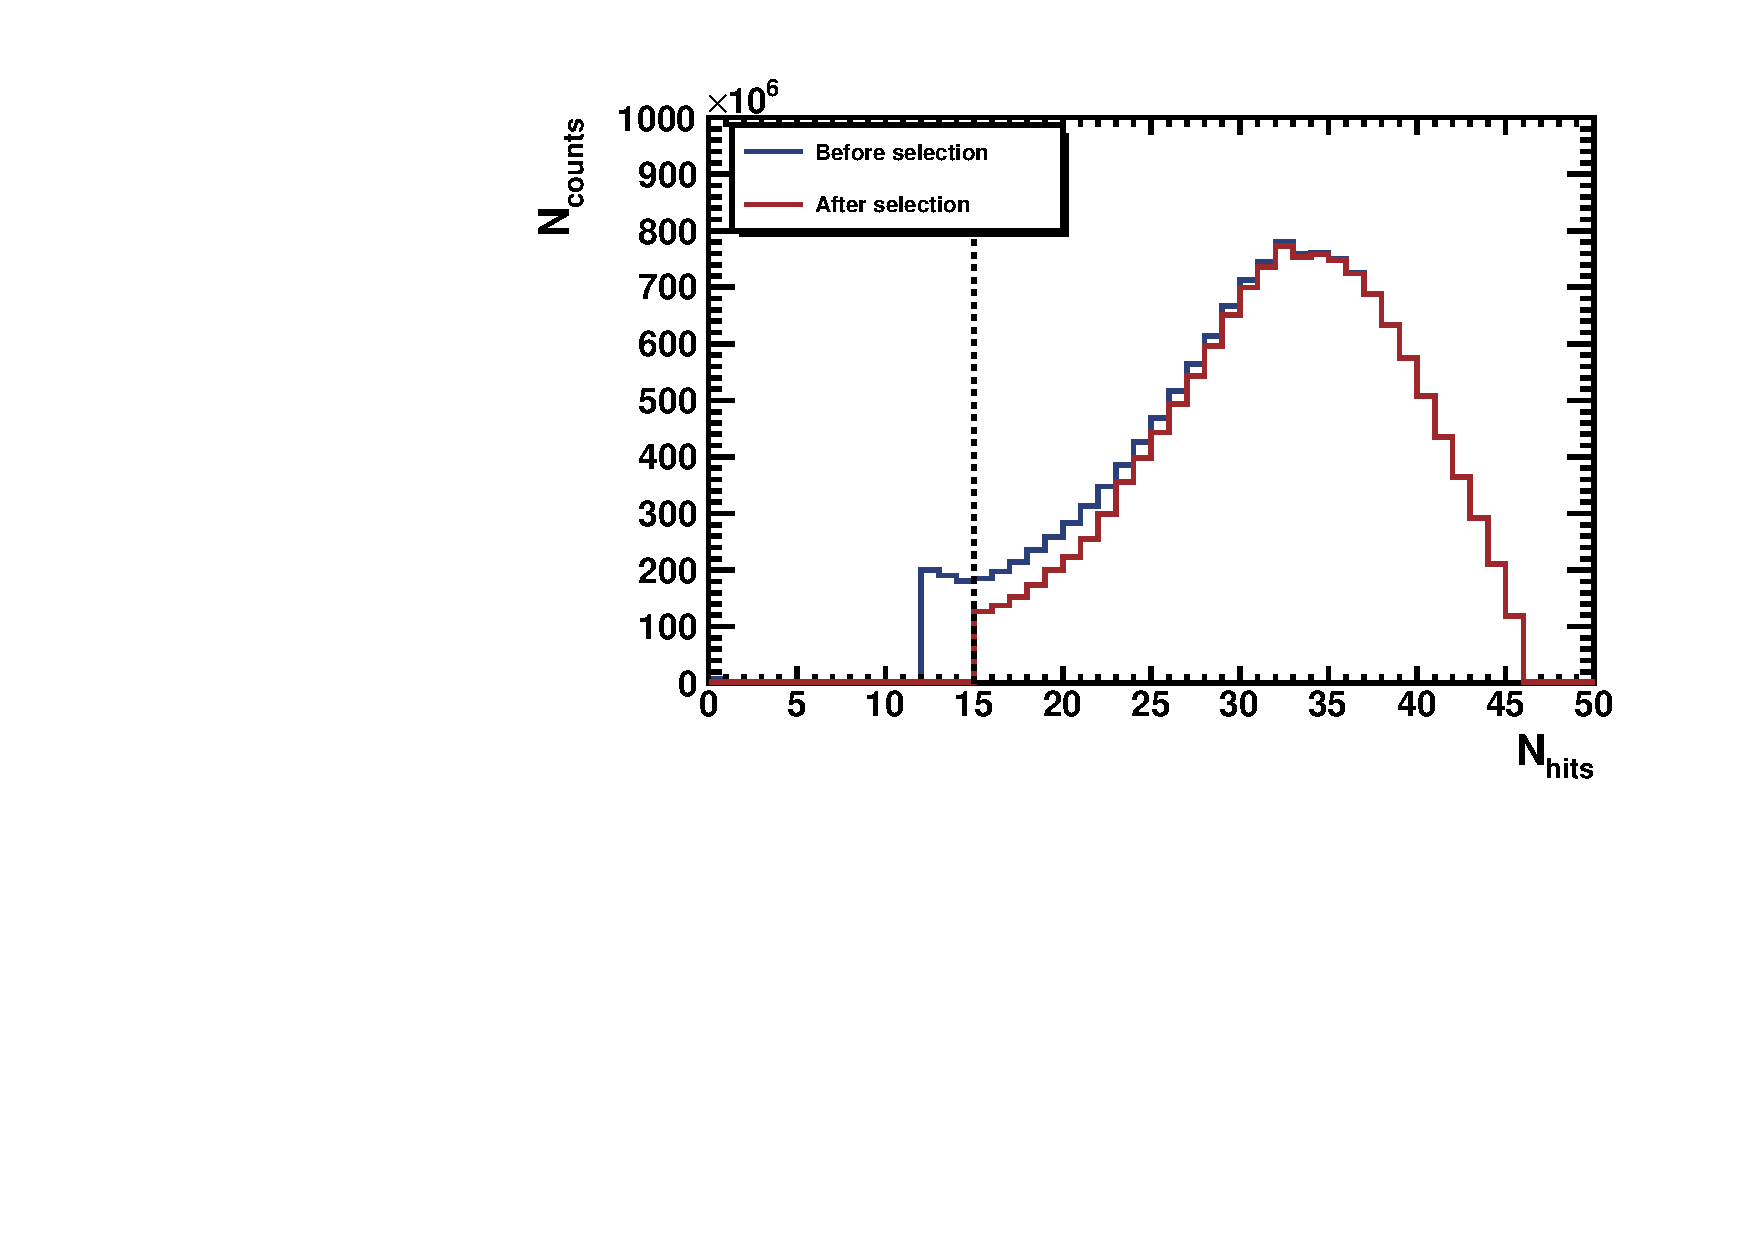
\includegraphics[width=0.49\textwidth]{Figures/Nhits.pdf}
    \end{multicols}
    \label{fig:TrackSelection}
    \caption{(upper left) $p_T$-distribution, (upper right) $|$\DCA$|$, (bottom left) $\eta$ and (bottom right) $N_{hits}$ distributions before and after track selection.}
\end{figure}

\FloatBarrier
\subsection {Particle identification}

\begin{figure}[ht]
    \begin{subfigure}{.49\textwidth}
        \centering
        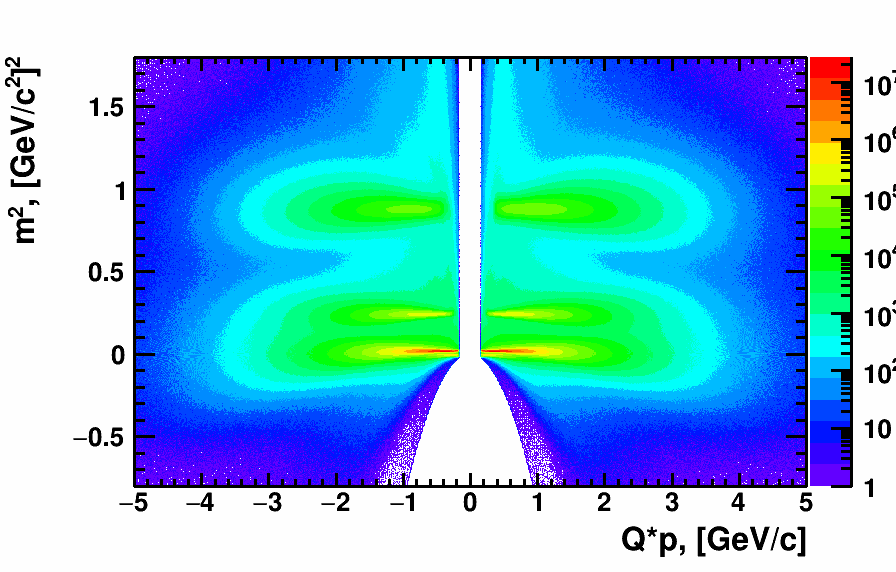
\includegraphics[width=1.\linewidth]{Figures/M2Qp_before_PID.png}
        %\caption{a}
    \end{subfigure}
    \begin{subfigure}{.49\textwidth}
        \centering
        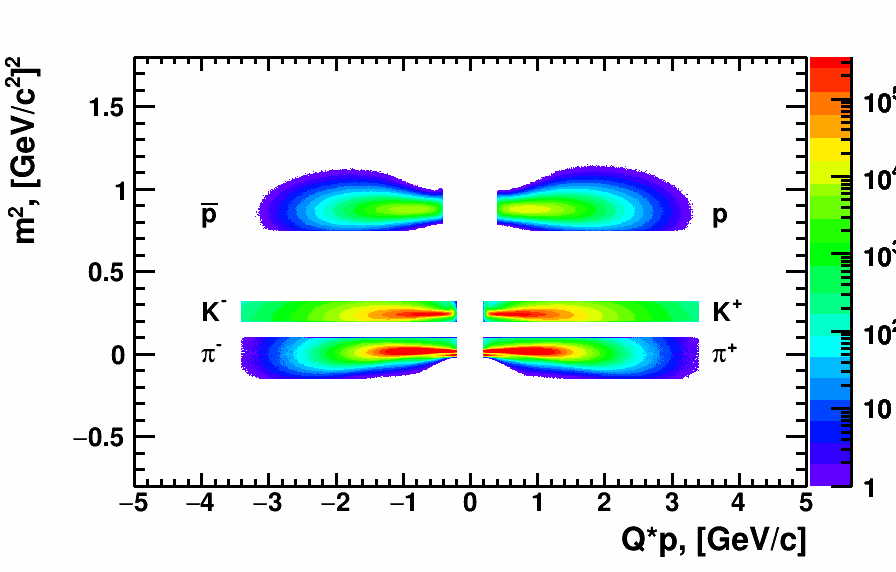
\includegraphics[width=1.\linewidth]{Figures/M2Qp_after_PID.png}
        %\caption{b}
    \end{subfigure}
    \label{fig:M2vsQp}
    \caption{$m^2$ estimated using \TPC\ and \TOF\ detectors vs charged total momentum $Q\cdot p$ before (left) and after (right) \PID\ procedure.}
\end{figure}